\documentclass[12pt,a4paper,oneside]{article}

\usepackage[utf8]{inputenc}
\usepackage[portuguese]{babel}
\usepackage[T1]{fontenc}
\usepackage{amsmath}
\usepackage{amsfonts}
\usepackage{amssymb}
\usepackage{graphicx}

\usepackage{xcolor}
% Definindo novas cores
\definecolor{verde}{rgb}{0.25,0.5,0.35}
\definecolor{jpurple}{rgb}{0.5,0,0.35}
% Configurando layout para mostrar codigos Java
\usepackage{listings}
\lstset{
  language=Java,
  basicstyle=\ttfamily\small, 
  keywordstyle=\color{jpurple}\bfseries,
  stringstyle=\color{red},
  commentstyle=\color{verde},
  morecomment=[s][\color{blue}]{/**}{*/},
  extendedchars=true, 
  showspaces=false, 
  showstringspaces=false, 
  numbers=left,
  numberstyle=\tiny,
  breaklines=true, 
  backgroundcolor=\color{cyan!10}, 
  breakautoindent=true, 
  captionpos=b,
  xleftmargin=0pt,
  tabsize=4,
  escapeinside=||
}

\author{\\Universidade Federal de Goiás (UFG) - Câmpus Jataí\\Bacharelado em Ciência da Computação \\Inteligência Artificial \\Esdras Lins Bispo Jr.}

\title{\sc \huge Segunda Prova}

\date{03 de abril de 2017}

\begin{document}

\maketitle

{\bf ORIENTAÇÕES PARA A RESOLUÇÃO}

\begin{itemize}
	\item A avaliação é individual, sem consulta;
	\item A pontuação máxima desta avaliação é 10,0 (dez) pontos, sendo uma das 04 (quatro) componentes que formarão a média final da disciplina: duas provas, um projeto e exercícios;
	\item A média final será calculada pela média ponderada das quatro supraditas notas [em que a primeira prova tem peso 35 (trinta e cinco), a segunda prova tem peso 25 (vinte e cinco), o projeto tem peso 30 (trinta) e os exercícios-bônus são adicionados à media final];
	\item O somatório da pontuação de todas as questões desta avaliação é 11,0 (onze) pontos. Isto é um sinônimo de tolerância na correção. Se você por acaso perder 1,5 (um e meio), sua nota será 9,5 (nove e meio);
	\item O conteúdo exigido compreende os seguintes pontos apresentados no Plano de Ensino da disciplina: (2) Agentes Inteligentes, (3) Resolução de Problemas, (6) Computação Natural, (7) Aprendizado de Máquina e (8) Mineração de dados.
\end{itemize}

\begin{center}
	\fbox{\large Nome: \hspace{10cm}}
	\fbox{\large Assinatura: \hspace{9cm}}
\end{center}

\newpage

\begin{enumerate}
	
	\item[] \colorbox{black}{
		\color{white}Todas as questões necessitam não apenas
	}\\ 
	\colorbox{black}{
		\color{white} serem respondidas, mas também justificadas.
	}

		\item (3,0 pt) [ENADE 2008] Considere um jogo do tipo 8-$puzzle$, cujo objetivo é conduzir o tabuleiro esquematizado na figura abaixo para o seguinte estado final. 
	
	\begin{center}
		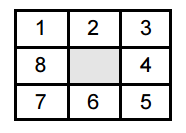
\includegraphics[width=4cm]{images/enade01.png}
	\end{center}
	
	Considere, ainda, que, em determinado instante do jogo, se tenha o estado $E0$ a seguir.
	
	\begin{center}
		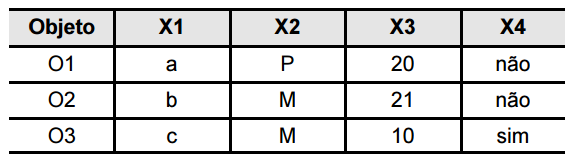
\includegraphics[width=4cm]{images/enade02.png}
	\end{center}
	
	Pelas regras desse jogo, sabe-se que os próximos estados possíveis são os estados $E1$, $E2$ e $E3$ mostrados abaixo.
	
	\begin{center}
		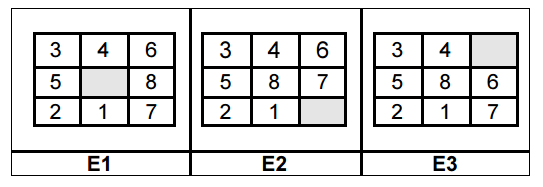
\includegraphics[width=10cm]{images/enade03.png}
	\end{center}
	
	Considere uma função heurística $h$ embasada na soma das distâncias das peças em relação ao estado final desejado,
	em que a distância $d$ a que uma peça $p$ está da posição final é dada pela soma do número de linhas com o número de colunas que a separam da posição final desejada. Por exemplo, em E1, $d(1) = 2 + 1 = 3$. A partir dessas informações analise as asserções a seguir.
	
	Utilizando-se um algoritmo de busca gulosa pela melhor escolha que utiliza a função h, o próximo estado no desenvolvimento do jogo a partir do estado $E0$ tem de ser $E3$.
	
	\begin{center}
		PORQUE
	\end{center}
	
	dos três estados $E1$, $E2$ e $E3$ possíveis, o estado com menor soma das distâncias entre a posição atual das peças e a posição final é o estado $E3$.
	
	\begin{enumerate}
		\item As duas asserções são proposições verdadeiras, e a segunda é uma justificativa correta da primeira.
		\item As duas asserções são proposições verdadeiras, e a segunda não é uma justificativa correta da primeira.
		\item A primeira asserção é uma proposição verdadeira, e a segunda é uma proposição falsa.
		\item A primeira asserção é uma proposição falsa, e a segunda é uma proposição verdadeira.
		\item As duas asserções são proposições falsas.
	\end{enumerate}	
	
	\item (2,5 pt) [ENADE 2008] Julgue os itens a seguir, relativos a métodos de busca com informação (busca heurística) e sem informação (busca cega), aplicados a problemas em que todas as ações têm o mesmo custo, o grafo de busca tem fator de ramificação finito e as ações não retornam a estados já visitados.
	
	\begin{enumerate}
		\item[] I - A primeira solução encontrada pela estratégia de busca em largura é a solução ótima. 
		\item[] II - A primeira solução encontrada pela estratégia de busca em profundidade é a solução ótima.
		\item[] III - As estratégias de busca com informação usam funções heurísticas que, quando bem definidas, permitem
		melhorar a eficiência da busca.
		\item[] IV - A estratégia de busca gulosa é eficiente porque expande apenas os nós que estão no caminho da
		solução.
	\end{enumerate}
	
	Estão certos apenas os itens:
	
	\begin{enumerate}
		\item I e II.
		\item I e III.
		\item I e IV.
		\item II e IV.
		\item III e IV.
	\end{enumerate}

	\item (2,5 pt) Escreva o pseudocódigo, tendo como base o algoritmo {\sc Intersect}, para os operadores do modelo de recuperação de informação booleano:
	\begin{enumerate}
		\item (1,0 pt) {\sc OR}($termo1$, $termo2$)
		\item (1,5 pt) {\sc XOR}($termo1$, $termo2$)
	\end{enumerate}
	
	\item (3,0 pt) O grafo abaixo mostra a ligação entre 5 cidades e as respectivas distâncias em quilômetros:
	
	\begin{center}
		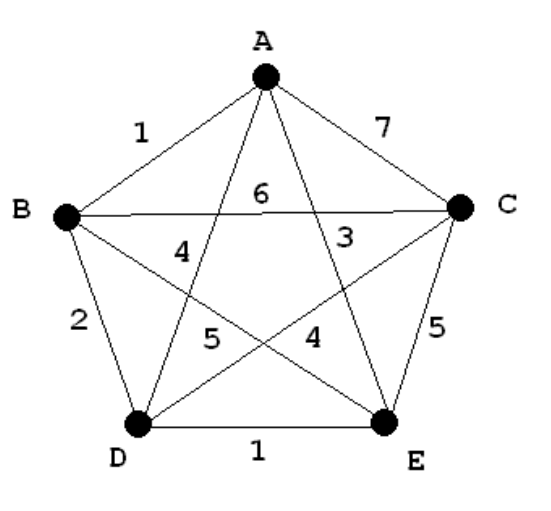
\includegraphics[width=5cm]{images/fig02.png}
	\end{center}
	
	Tem-se um problema em que é necessário passar por todas as cidades, apenas uma vez. O objetivo é encontrar uma rota de menor custo usando um algoritmo genético.
	
	\begin{enumerate}
		\item (0,5 pt) Proponha uma maneira de codificar os cromossomos.
		\item (0,5 pt) Defina uma função de aptidão para avaliar a qualidade dos cromossomos.
		\item (0,5 pt) Gere dois cromossomos e avalie a aptidão deles.
		\item (0,5 pt) Realize o cruzamento entre os cromossomos.
		\item (0,5 pt) Aplique uma mutação em um gene dos cromossomos.
		\item (0,5 pt) Aplique a função de aptidão nos descendentes gerados verificando se a solução encontrada é melhor ou não.
	\end{enumerate}
	
	\end{enumerate}
\end{document}